\documentclass[tikz,border=5pt]{standalone}
\usepackage{fontspec}
\setmainfont{Times New Roman}
\usepackage{unicode-math}
\setmathfont{Cambria Math}
\usetikzlibrary{shapes.geometric,positioning,fit,backgrounds,arrows.meta,calc}

\begin{document}
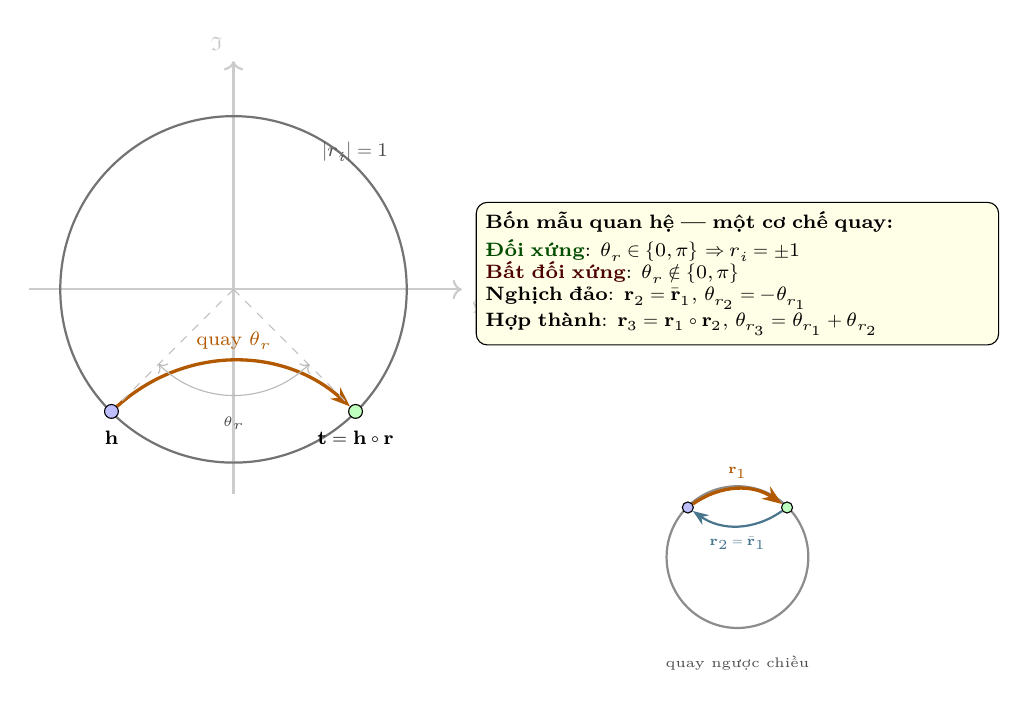
\begin{tikzpicture}[
  pt/.style={circle, draw, fill=blue!10, inner sep=1.5pt, minimum size=5pt},
  arrow/.style={-{Stealth[length=2.5mm]}, thick},
  rot/.style={-{Stealth[length=2.5mm]}, very thick, orange!70!black},
  label/.style={font=\scriptsize\itshape, text=gray!60!black},
  pat/.style={font=\scriptsize, align=left},
]

% ====== Unit circle (complex plane) ======
\draw[->, gray!40, thick] (-2.6, 0) -- (2.9, 0) node[below right, font=\scriptsize\color{gray!60!black}] {$\Re$};
\draw[->, gray!40, thick] (0, -2.6) -- (0, 2.9) node[above left, font=\scriptsize\color{gray!60!black}] {$\Im$};
\draw[thick, black!55] (0,0) circle (2.2);
\node[label] at (1.55, 1.75) {$|r_i| = 1$};

% ====== Entity h and rotated t = h o r ======
\node[pt, fill=blue!25] (h) at (-1.55, -1.55) {};
\node[pt, fill=green!25] (t) at (1.55, -1.55) {};
\node[font=\scriptsize, below=1pt of h] {$\mathbf{h}$};
\node[font=\scriptsize, below=1pt of t] {$\mathbf{t}=\mathbf{h}\circ\mathbf{r}$};
\draw[rot] (h) to[bend left=42] node[midway, above, font=\scriptsize, text=orange!70!black] {quay $\theta_r$} (t);
\draw[dashed, gray!50] (0,0) -- (h);
\draw[dashed, gray!50] (0,0) -- (t);
\draw[<->, gray!55] (-0.95, -0.95) arc (225:315:1.35);
\node[font=\tiny, text=gray!55!black] at (0, -1.7) {$\theta_r$};

% ====== Four relational patterns ======
\node[draw, rounded corners, fill=yellow!10, align=left, font=\scriptsize, text width=6.4cm]
  (legend) at (6.4, 0.2)
  {\textbf{Bốn mẫu quan hệ — một cơ chế quay:}\\[2pt]
   \textcolor{black!70!green}{\textbf{Đối xứng}}: $\theta_r \in \{0,\pi\}$ $\Rightarrow r_i=\pm1$\\
   \textcolor{black!70!red}{\textbf{Bất đối xứng}}: $\theta_r \notin \{0,\pi\}$\\
   \textbf{Nghịch đảo}: $\mathbf{r}_2=\bar{\mathbf{r}}_1$, $\theta_{r_2}=-\theta_{r_1}$\\
   \textbf{Hợp thành}: $\mathbf{r}_3=\mathbf{r}_1\circ\mathbf{r}_2$, $\theta_{r_3}=\theta_{r_1}+\theta_{r_2}$};

% ====== Inversion mini-diagram ======
\begin{scope}[shift={(6.4,-3.4)}]
  \draw[thick, black!45] (0,0) circle (0.9);
  \node[pt, fill=blue!25, inner sep=1pt, minimum size=4pt] (a) at (-0.63,0.63) {};
  \node[pt, fill=green!25, inner sep=1pt, minimum size=4pt] (b) at (0.63,0.63) {};
  \draw[rot] (a) to[bend left=35] node[above, font=\tiny] {$\mathbf{r}_1$} (b);
  \draw[-{Stealth[length=2mm]}, thick, cyan!50!black] (b) to[bend left=35] node[below, font=\tiny, text=cyan!50!black] {$\mathbf{r}_2=\bar{\mathbf{r}}_1$} (a);
  \node[font=\tiny, text=gray!60!black] at (0,-1.35) {quay ngược chiều};
\end{scope}

\end{tikzpicture}
\end{document}
